\slide{Definição do Cenário}{
    \begin{itemize}
        \item Fator Espacial
        \item Fator Temporal
        \item Fator Aleatório
        \item Dados de Maio a Junho de 2016
    \end{itemize}
}

\slide{Tratamento dos Dados}{
Inicialmente, os dados possuíam algumas inconsistências. Algumas das colunas também não eram necessárias para o problema, por isso foram removidas:
    \begin{itemize}
        \item Faixa
        \item Hora
        \item Tamanho do Veículo (inconsistente)
    \end{itemize}
}

\slide{Transformação dos Dados}{
A coluna \textit{Data} teve o seu formato alterado para melhorar o treinamento dos modelos e evitar falsas suposições devido ao formato original dos dados. Para realizar a transformação utilizou-se \textit{One Hot Enconding}
    \begin{itemize}
        \item Ex: Segunda-Feira = [0][1][0][0][0][0][0]
        \item Ex: Terça-Feira = [0][0][1][0][0][0][0]
    \end{itemize}
}

\slide{Transformação dos Dados}{
Com todas as colunas no formato adequado, o conjunto de registro de veículos foi transformado em um conjunto de acumulação de fluxo de veículos.

    \begin{itemize}
      \item Acumulo de 2.5, 5 e 7.5 minutos;
      \item Cáculo da densidade;
      \item Cáculo da velocidade média
    \end{itemize}
}


\slide{Dados após tratamento completo}{
    \begin{figure}[htbp]
        \centering
        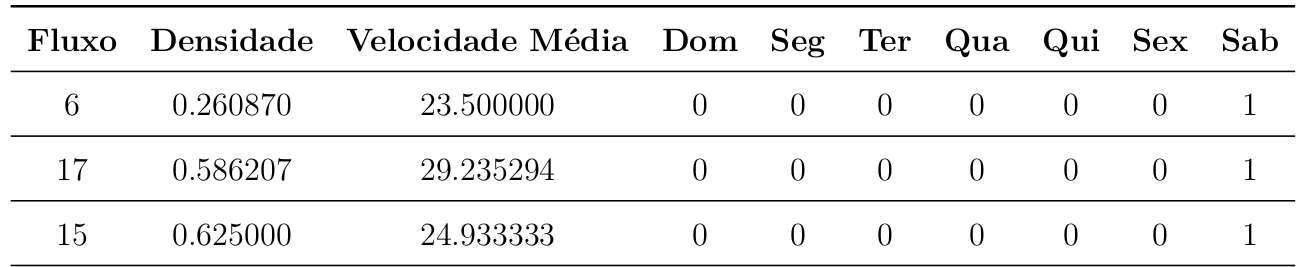
\includegraphics[scale=2,7]{presentation/img/acumuloFluxo.png}
    \end{figure}
}

\slide{Treino}{
    \begin{itemize}
        \item Memória do Passado
        \item Univariado
        \item Multivariado
        \item Janela Rolante de Treino
    \end{itemize}
}

\slide{Escolha dos Parâmetros e Hiper-parâmetros}{
    Parâmetros Gerais:
    \begin{itemize}
        \item Memória do Passado \textbf{(1h a 8h, 1h)}
        \item Janela de Treino \textbf{(0.30 a 0.80, 0.05)}
    \end{itemize}
}

\slide{Escolha dos Parâmetros e Hiper-parâmetros}{
    Específicos de Aprendizagem Profunda:
    \begin{itemize}
        \item Quantidade de Neurônios \textbf{(40 a 200, 10)}
        \item Funções de Ativação \textbf{(Sigmoid, ReLu e Softmax)}
        \item Otimizador do Modelo \textbf{(Adam, Adamax)} % https://keras.io/optimizers/
    \end{itemize}
}

\slide{Escolha dos Parâmetros e Hiper-parâmetros}{
    Específicos de Random Forest:
    \begin{itemize}
        \item Números de Estimadores \textbf{(50 a 400, 50)}
        %\item Altura Máxima \textbf{(TODO)}
        \item Bootstrapping \textbf{(True ou False)}
    \end{itemize}
}

\slide{Escolha dos Parâmetros e Hiper-parâmetros}{
    Específicos de SVM:
    \begin{itemize}
        \item TODO!
    \end{itemize}
}

\slide{Métricas de Avaliação}{
    \begin{itemize}
        \item Raiz do Erro Médio Quadrádico
        \item Raiz do Erro Médio Quadrádico Normalizado
        \item Erro Máximo Absoluto
        \item Precisão de Tendência
    \end{itemize}
}